\documentclass[10pt,xcolor=table]{beamer}

\usetheme[progressbar=frametitle]{metropolis}
\usepackage{appendixnumberbeamer}
\usepackage{hyperref}
\usepackage{tikz}
\usetikzlibrary{calc,decorations.pathreplacing,snakes}
\usepackage{multicol}
\usepackage{comment}
\usepackage[portuguese]{babel}
\usepackage[style=authortitle,backend=bibtex]{biblatex}
\addbibresource{references.bib}
\usepackage{subfig}

\hypersetup{colorlinks=true,linkcolor=,urlcolor=blue}

\expandafter\def\expandafter\insertshorttitle\expandafter{%
  \insertshorttitle\hfill%
  \insertframenumber\,/\,\inserttotalframenumber}

\newcommand{\hideFromPandoc}[1]{#1}
\hideFromPandoc{
  \let\Begin\begin
  \let\End\end
}

\newcommand{\verbatimfont}[1]{\renewcommand{\verbatim@font}{\ttfamily#1}}

\newcommand{\PR}[1]{\ensuremath{\left[#1\right]}}
\newcommand{\PC}[1]{\ensuremath{\left(#1\right)}}
\newcommand{\chav}[1]{\ensuremath{\left\{#1\right\}}}

\usepackage{booktabs}
\usepackage[scale=2]{ccicons}

\usepackage{pgfpages} % for multiple-screen presentations
% \setbeameroption{show notes on second screen}
% \setbeameroption{show notes on second screen=right} % Both

\usepackage{pgfplots}
\usepgfplotslibrary{dateplot}

\usepackage{xspace}
\newcommand{\themename}{\textbf{\textsc{metropolis}}\xspace}

\setbeamertemplate{frame footer}{
\includegraphics[height=0.65cm]{figs/ifpb.png}}

\setbeamercolor{background canvas}{bg=white}

% \setbeamertemplate{sections/subsections in toc}[ball]
\setbeamertemplate{section in toc}[sections numbered]
\setbeamertemplate{subsection in toc}[ball unnumbered]
\setbeamerfont{footnote}{size=\scriptsize}

% \renewcommand{\footnotesize}{\small}
\renewcommand*{\bibfont}{\tiny}

% Slide de Título
\title{Integração do 5G com Tecnologias Habilitadoras nas Telecomunicações}
% \subtitle{Subtítulo}
\date{\today}
% \date{}
\author{\textbf{Prof. Paulo Ditarso Maciel Jr.}}
\institute{
\centering
\normalsize
\textbf{Programa de Pós-Graduação em Engenharia Elétrica (PPGEE)}\\
\vspace{0.3cm}
\textbf{Aula Inaugural do PPGEE -- Turma 2024.2}
}


\titlegraphic{\hfill
\includegraphics[height=1.7cm]{figs/ifpb.png}}


\begin{document}

\maketitle

% Slide de Título
\begin{frame}
    \frametitle{Atenção\footnote{Todas as figuras usadas nesta apresentação estão disponíveis publicamente em artigos científicos ou são licenciadas pela \textit{Creative Commons}.}}
    \begin{itemize}
        \item Esta apresentação não pretende aprofundar nenhum tópico!
        \item E qual é o objetivo desta apresentação?
    \end{itemize}
    \begin{figure}
        \centering
        \includegraphics[width=0.6\textwidth]{figs/Interrogacao.jpg}
    \end{figure}
    \note{Não sou da área de telecomunicações, meu background é na área de redes de computadores, mais especificamente, na subárea de gerência de redes. Alocar e utilizar os recursos eficientemente.}
    % \vspace{2cm}
\end{frame}

% Slide de Agenda
\begin{frame}
    \frametitle{Agenda}
    \tableofcontents
\end{frame}

% Seção 1: Introdução às Redes 5G

\section{Introdução às Redes 5G}
\begin{frame}
    \frametitle{O que é o 5G?}
    \begin{itemize}
        \item Quinta geração de redes móveis.
        \item Promete velocidades ultrarrápidas, latência ultrabaixa e conectividade massiva.
        \item Suporte a novas aplicações, como IoT, realidade aumentada/virtual, veículos autônomos.
    \end{itemize}
\end{frame}

\begin{frame}
    \frametitle{Arquitetura do 5G}
    \begin{itemize}
        \item \textbf{Rede de Acesso por Rádio (RAN)}: Nova radiofrequência e técnicas avançadas de transmissão.
        \item \textbf{Rede Central (Core)}: Baseada em software, mais flexível e ágil.
        \item \textbf{Suporte Multisserviço}: Network slicing para diferentes tipos de serviços.
    \end{itemize}
    \begin{figure}
        \centering
        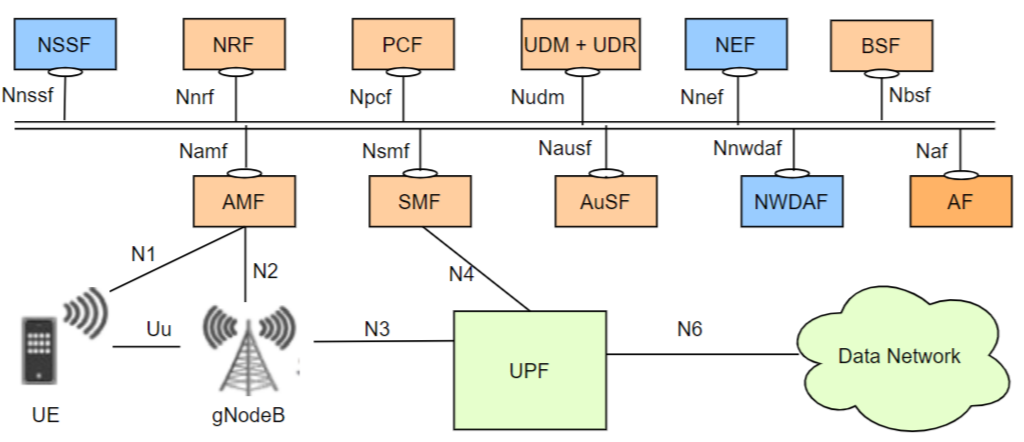
\includegraphics[width=0.7\textwidth]{figs/ArquiteturaGeral5G}
        \caption{Arquitetura Geral do 5G\footcite{5G_architecture}}
    \end{figure}
\end{frame}

\begin{frame}
    \frametitle{Características Técnicas do 5G}
    \begin{itemize}
        \item \textbf{Velocidade}: Até 20 Gbps.
        \item \textbf{Latência}: Menos de 1 ms.
        \item \textbf{Conectividade Massiva}: Suporte para até 1 milhão de dispositivos por km².
        \item \textbf{Eficiência Espectral}: Utilização otimizada do espectro.
    \end{itemize}
    \begin{figure}
        \centering
        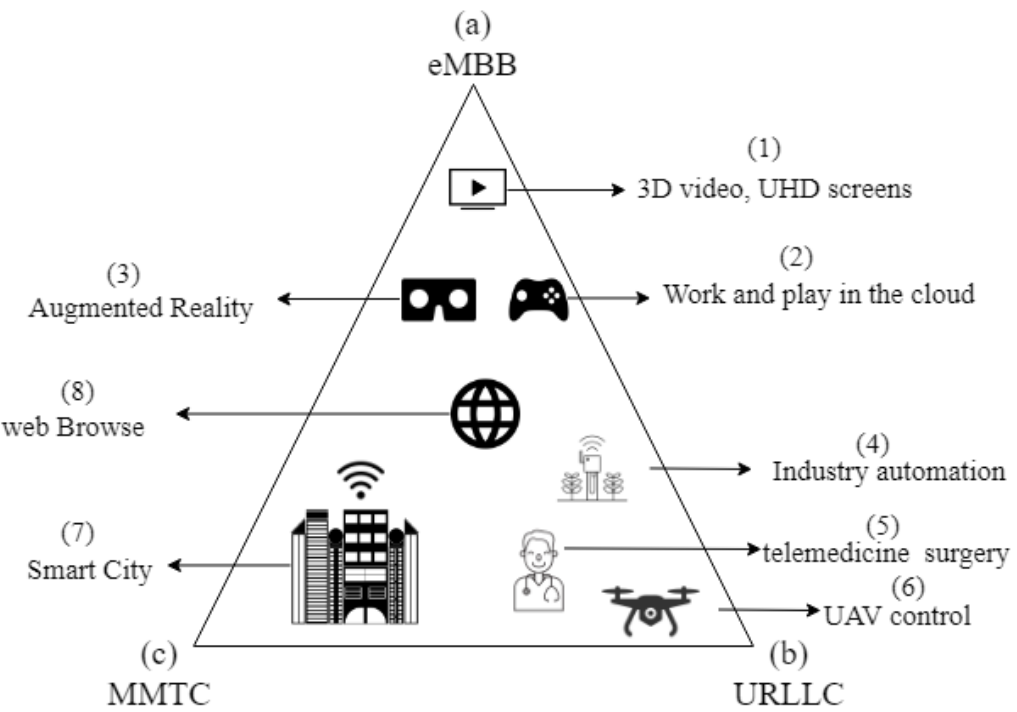
\includegraphics[width=0.5\linewidth]{figs/5G_verticais.png}
        \caption{Requisitos para diferentes tipos de aplicações\footcite{5G_verticais}}
        \label{fig:enter-label}
    \end{figure}
\end{frame}


% Seção 2: Tecnologias Habilitadoras do 5G

\section{Tecnologias Habilitadoras do 5G}
\subsection{Redes Definidas por Software (SDN)}

\begin{frame}
    \frametitle{Introdução ao SDN}

    \begin{itemize}
        \item \textbf{Definição}: Arquitetura de rede que separa o plano de controle do plano de dados.
        \item \textbf{Componentes Principais}: Aplicações de rede, controlador SDN, switches programáveis, interfaces.
        \item \textbf{Vantagens}: Flexibilidade, centralização do controle, automação.
    \end{itemize}
    \begin{figure}
        \centering
        \subfloat[Tradicional]{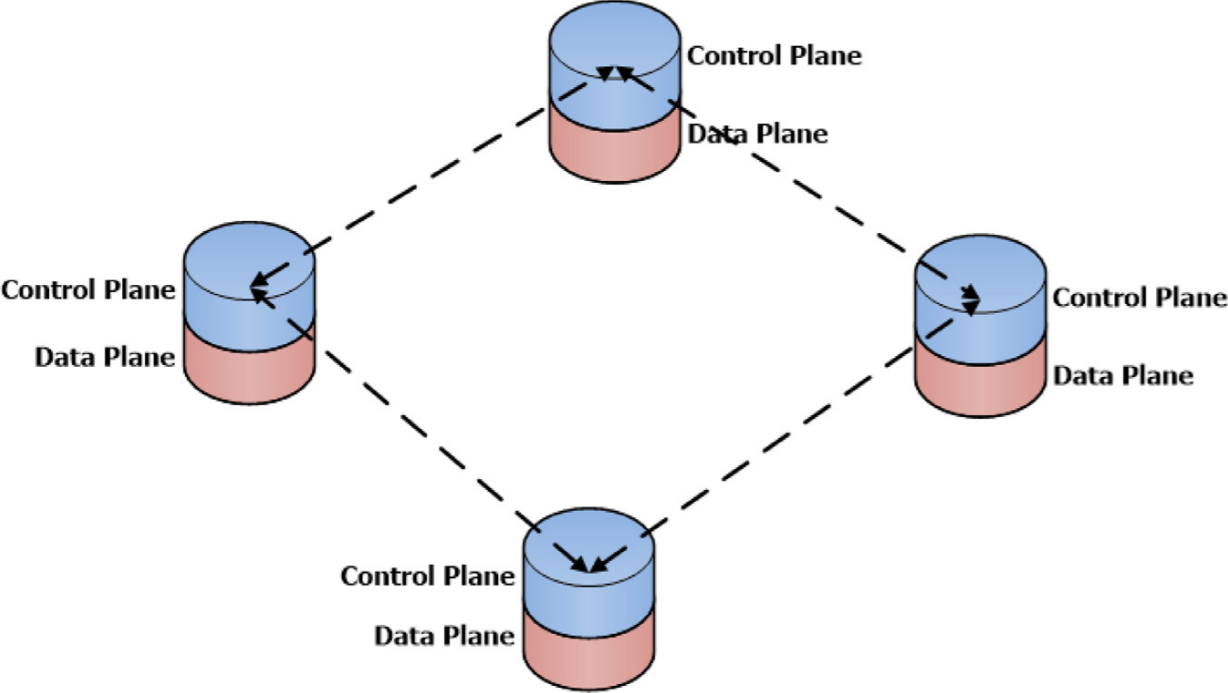
\includegraphics[width=0.45\linewidth]{figs/rede_tradicional.png}}\qquad
        \subfloat[SDN]{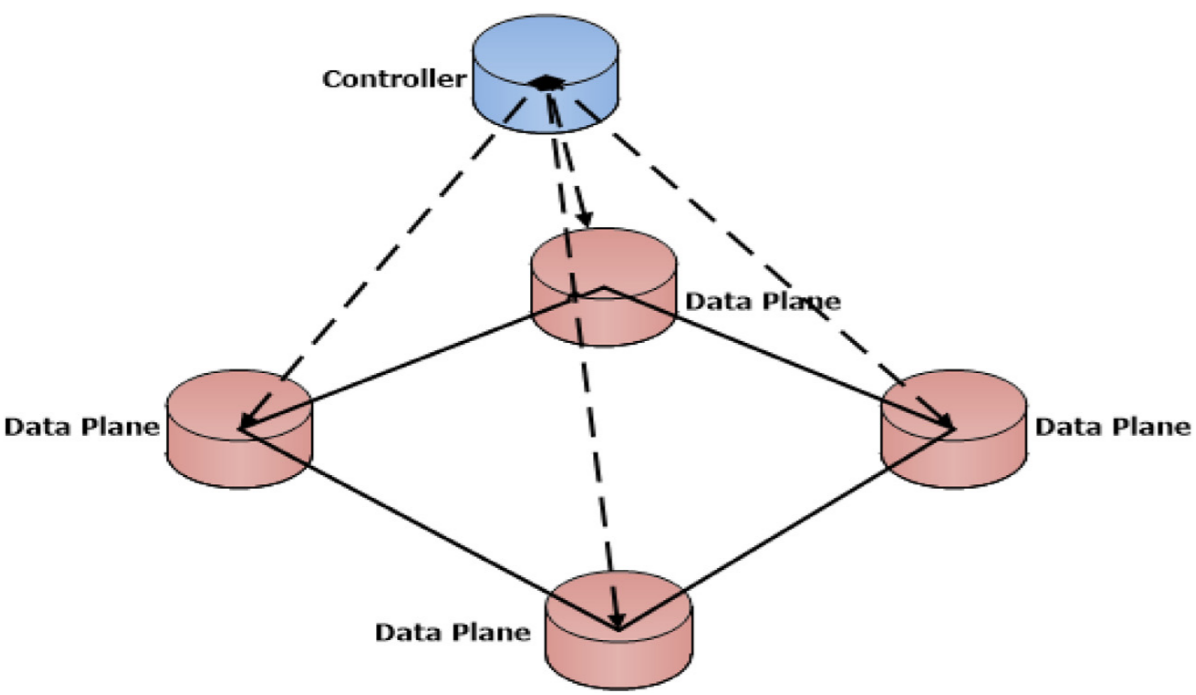
\includegraphics[width=0.45\linewidth]{figs/rede_sdn.png}}
        \caption{Redes tradicionais vs SDN\footcite{Plane_Separation}}
        \end{figure}
\end{frame}

\begin{frame}
    \frametitle{Componentes SDN}
    \begin{columns}
        \begin{column}{0.55\textwidth}
            \begin{itemize}
                \item \textbf{Plano de Aplicação}: Controle dos recursos via programação.
                \item \textbf{Plano de Controle}: Gerência centralizada dos recursos de rede.
                \item \textbf{Plano de Dados}: Dispositivos de comutação físicos ou virtuais.
                \item \textbf{Interfaces}: Comunicação entre os planos, ao norte (REST), sul (OpenFlow, P4), leste, oeste (API dos controladores).
        \end{itemize}            
        \end{column}
        \begin{column}{0.45\textwidth}
            \vspace{1cm}
            \begin{figure}[h]
                \centering
                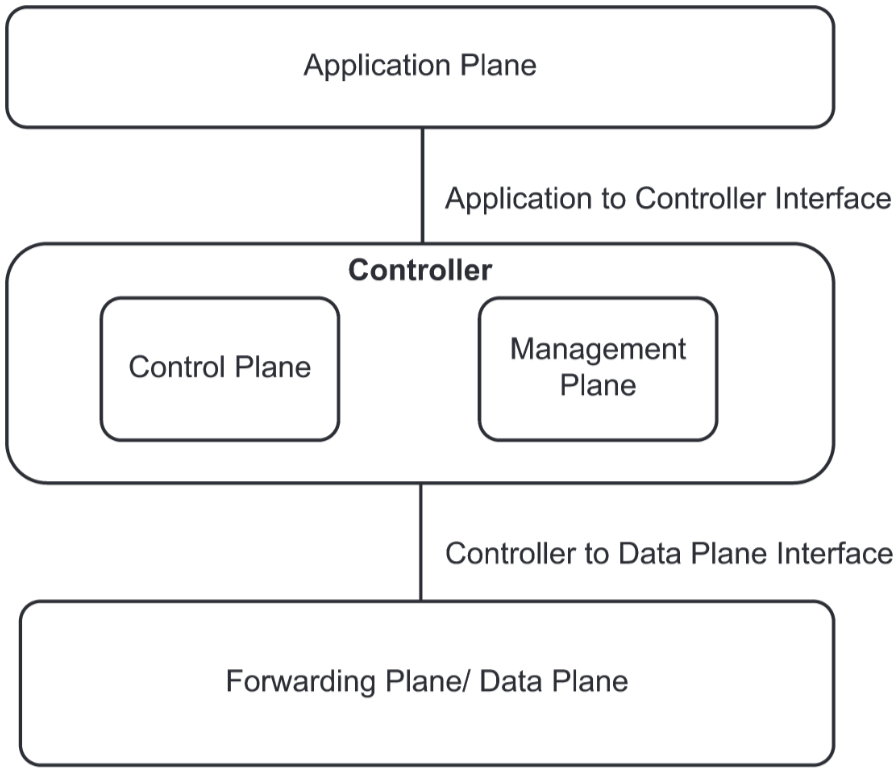
\includegraphics[width=\textwidth]{figs/SDN_arquitetura.png}
                \caption{Arquitetura SDN\footcite{Recommended_SDN_Wireless}}
            \end{figure}
        \end{column}
    \end{columns}
\end{frame}

\begin{frame}
    \frametitle{Integração SDN com 5G}
    \begin{itemize}
        \item \textbf{Automação de Redes}: Gerência dinâmica do tráfego e recursos.
        \item \textbf{Casos de Uso}: Redes IoT, redes industriais, redes de campus.
        \item \textbf{\textit{Network Slicing}}: Criação de fatias para diferentes serviços.
    \end{itemize}
\end{frame}

\subsection{Virtualização das Funções de Rede (NFV)}
\begin{frame}
    \frametitle{Introdução ao NFV}
    \begin{itemize}
        \item \textbf{Definição}: Abstração das funções de rede do hardware proprietário, executando-as em servidores padrão.
        \item \textbf{Componentes Principais}: VNF (Funções de Rede Virtualizadas), NFVI (Infraestrutura de Virtualização).
        \item \textbf{Vantagens}: Redução de custos, flexibilidade, rapidez na introdução de serviços.
    \end{itemize}
    % \begin{figure}
    %     \centering
    %     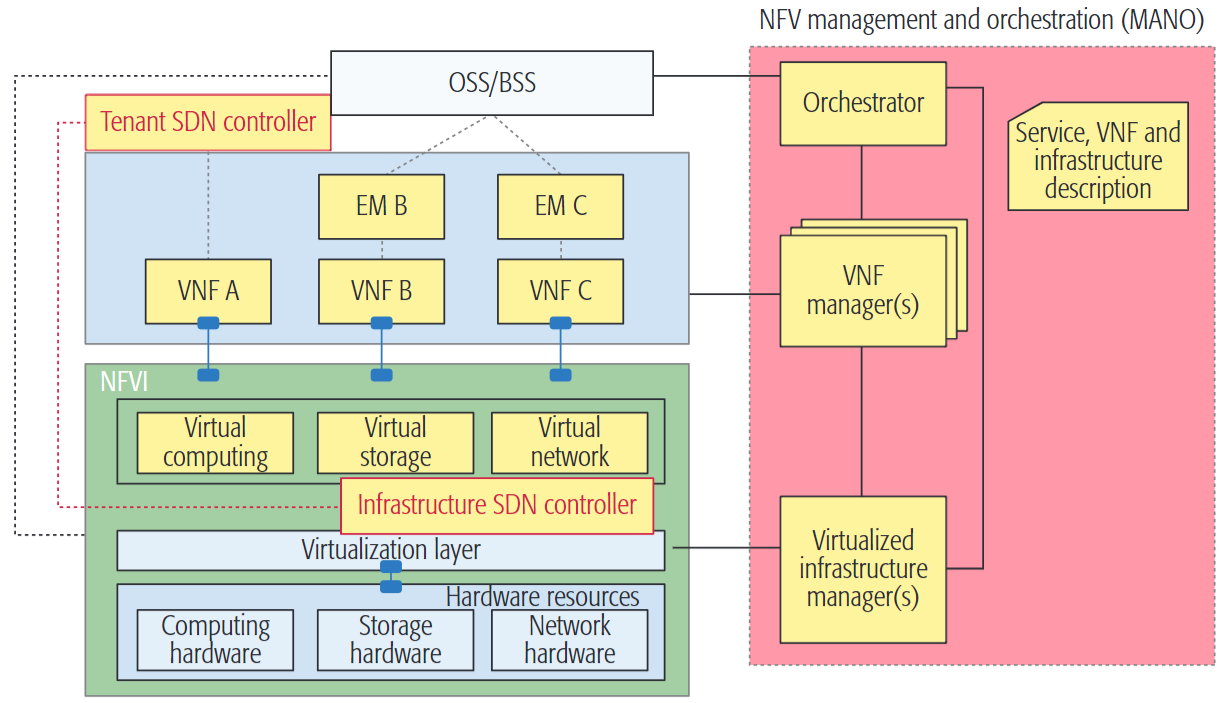
\includegraphics[width=0.5\linewidth]{figs/ArquiteturaNFV.png}
    %     \caption{Arquitetura geral NFV}
    % \end{figure}
\end{frame}

\begin{frame}
    \frametitle{Integração NFV com 5G}
    \begin{itemize}
        \item \textbf{Virtualização do EPC (\textit{Evolved Packet Core})}: Gestão centralizada e flexível do core da rede.
        \item \textbf{vRAN (\textit{Virtualized Radio Access Network})}: Otimização da rede de acesso rádio.
        \item \textbf{\textit{Edge Computing}}: Suporte a aplicações de baixa latência e alta demanda.
    \end{itemize}
\end{frame}

\subsection{\textit{Network Slicing} (NS)}
\begin{frame}
    \frametitle{Introdução ao \textit{Network Slicing}}
    \begin{itemize}
        \item \textbf{Definição}: Técnica que permite a criação de múltiplas redes virtuais independentes sobre uma única infraestrutura física, otimizadas para atender diferentes requisitos de serviços e aplicações dentro de uma rede 5G.
        \item \textbf{Componentes Principais}: NFV e SDN.
        \item \textbf{Vantagens}: Garantir QoS, agilidade de implantação, personalizar e otimizar recursos de rede para diferentes serviços.
    \end{itemize}
\end{frame}

\begin{frame}{Integração NS com 5G}
    \begin{figure}[h]
        \centering
        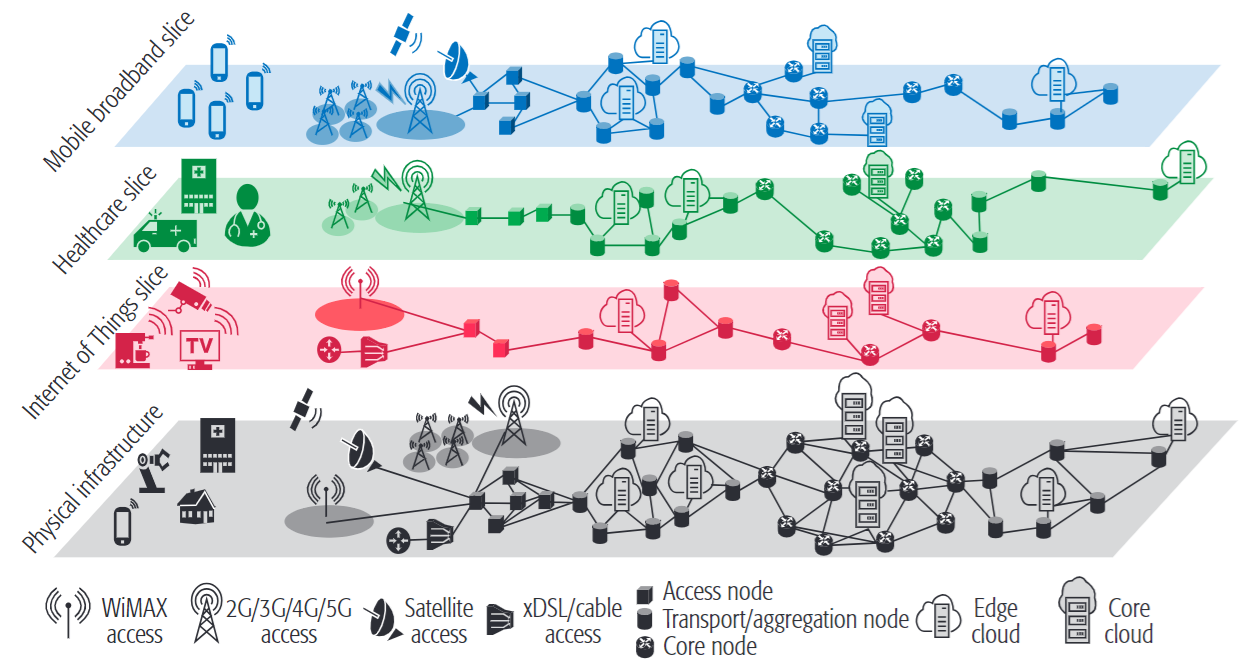
\includegraphics[width=\textwidth]{figs/Network_Slicing.png}
        \caption{Fatiamento de redes\footcite{Network_Slicing}}
    \end{figure}
\end{frame}

% Seção 3: Controle de Loop Fechado

\section{Controle de Loop Fechado no 5G}
\begin{frame}
    \frametitle{O que é Controle de Loop Fechado?}
    \begin{itemize}
        \item \textbf{Definição}: Sistema de automação que ajusta parâmetros da rede em tempo real com base em feedback contínuo.
        \item \textbf{Componentes}: Monitoramento, análise, decisão e execução.
        \item \textbf{Benefícios}: Otimização contínua da rede, melhoria na Qualidade de Serviço (QoS), resposta rápida a falhas.
    \end{itemize}
\end{frame}

\begin{frame}
    \frametitle{Aplicações do Controle de Loop Fechado no 5G}
    \begin{itemize}
        \item \textbf{Self-Organizing Networks (SON)}: Redes que se auto-configuram, otimizam e recuperam.
        \item \textbf{Gerenciamento de Tráfego}: Ajustes automáticos para otimizar o fluxo de dados.
        \item \textbf{Manutenção Preditiva}: Prevenção de falhas com base em análise contínua de dados.
    \end{itemize}
\end{frame}

% Seção 4: Indústria 4.0 e 5G
\section{Indústria 4.0 e 5G}
\begin{frame}
    \frametitle{Introdução à Indústria 4.0}
    \begin{itemize}
        \item \textbf{Definição}: Fusão de tecnologias digitais, físicas e biológicas, impulsionada pela conectividade e automação.
        \item \textbf{Componentes}: IoT, robótica avançada, big data, IA, e computação em nuvem.
        \item \textbf{Objetivo}: Produção mais inteligente, eficiente e flexível.
    \end{itemize}
\end{frame}

\begin{frame}
    \frametitle{O Papel do 5G na Indústria 4.0}
    \begin{itemize}
        \item \textbf{Conectividade Onipresente}: Conexão confiável para um grande número de dispositivos e sensores.
        \item \textbf{Baixa Latência}: Comunicação quase em tempo real, essencial para automação.
        \item \textbf{Customização e Flexibilidade}: Produção adaptável às demandas do mercado.
    \end{itemize}
 %    \begin{figure}
 %        \centering
 %        \fbox{
	%    \begin{minipage}{1in}
	% 	  \hfill\vspace{1in}
	%    \end{minipage}
	% }
 %        \caption{5G e Indústria 4.0}	
 %    \end{figure}
    % \begin{figure}[h]
    %     \centering
    %     \includegraphics[width=0.8\textwidth]{Industry_4.0.png}
    %     \caption{5G e Indústria 4.0}
    % \end{figure}
\end{frame}

\begin{frame}
    \frametitle{Casos de Uso do 5G na Indústria 4.0}
    \begin{itemize}
        \item \textbf{Automação e Robótica}: Robôs conectados em tempo real.
        \item \textbf{Manutenção Preditiva}: Monitoramento contínuo de equipamentos para prever falhas.
        \item \textbf{Supply Chain Inteligente}: Integração e otimização em tempo real de toda a cadeia de suprimentos.
    \end{itemize}
\end{frame}



% Seção 5: Pesquisa Autoral
\section{Pesquisa Autoral}
\begin{frame}{Disseminação de Eventos Críticos por VANETS\footcite{Andrade2021a,Andrade2021b}}
    \begin{columns}
        \begin{column}{0.65\textwidth}
            \begin{figure}
                \centering
                \subfloat{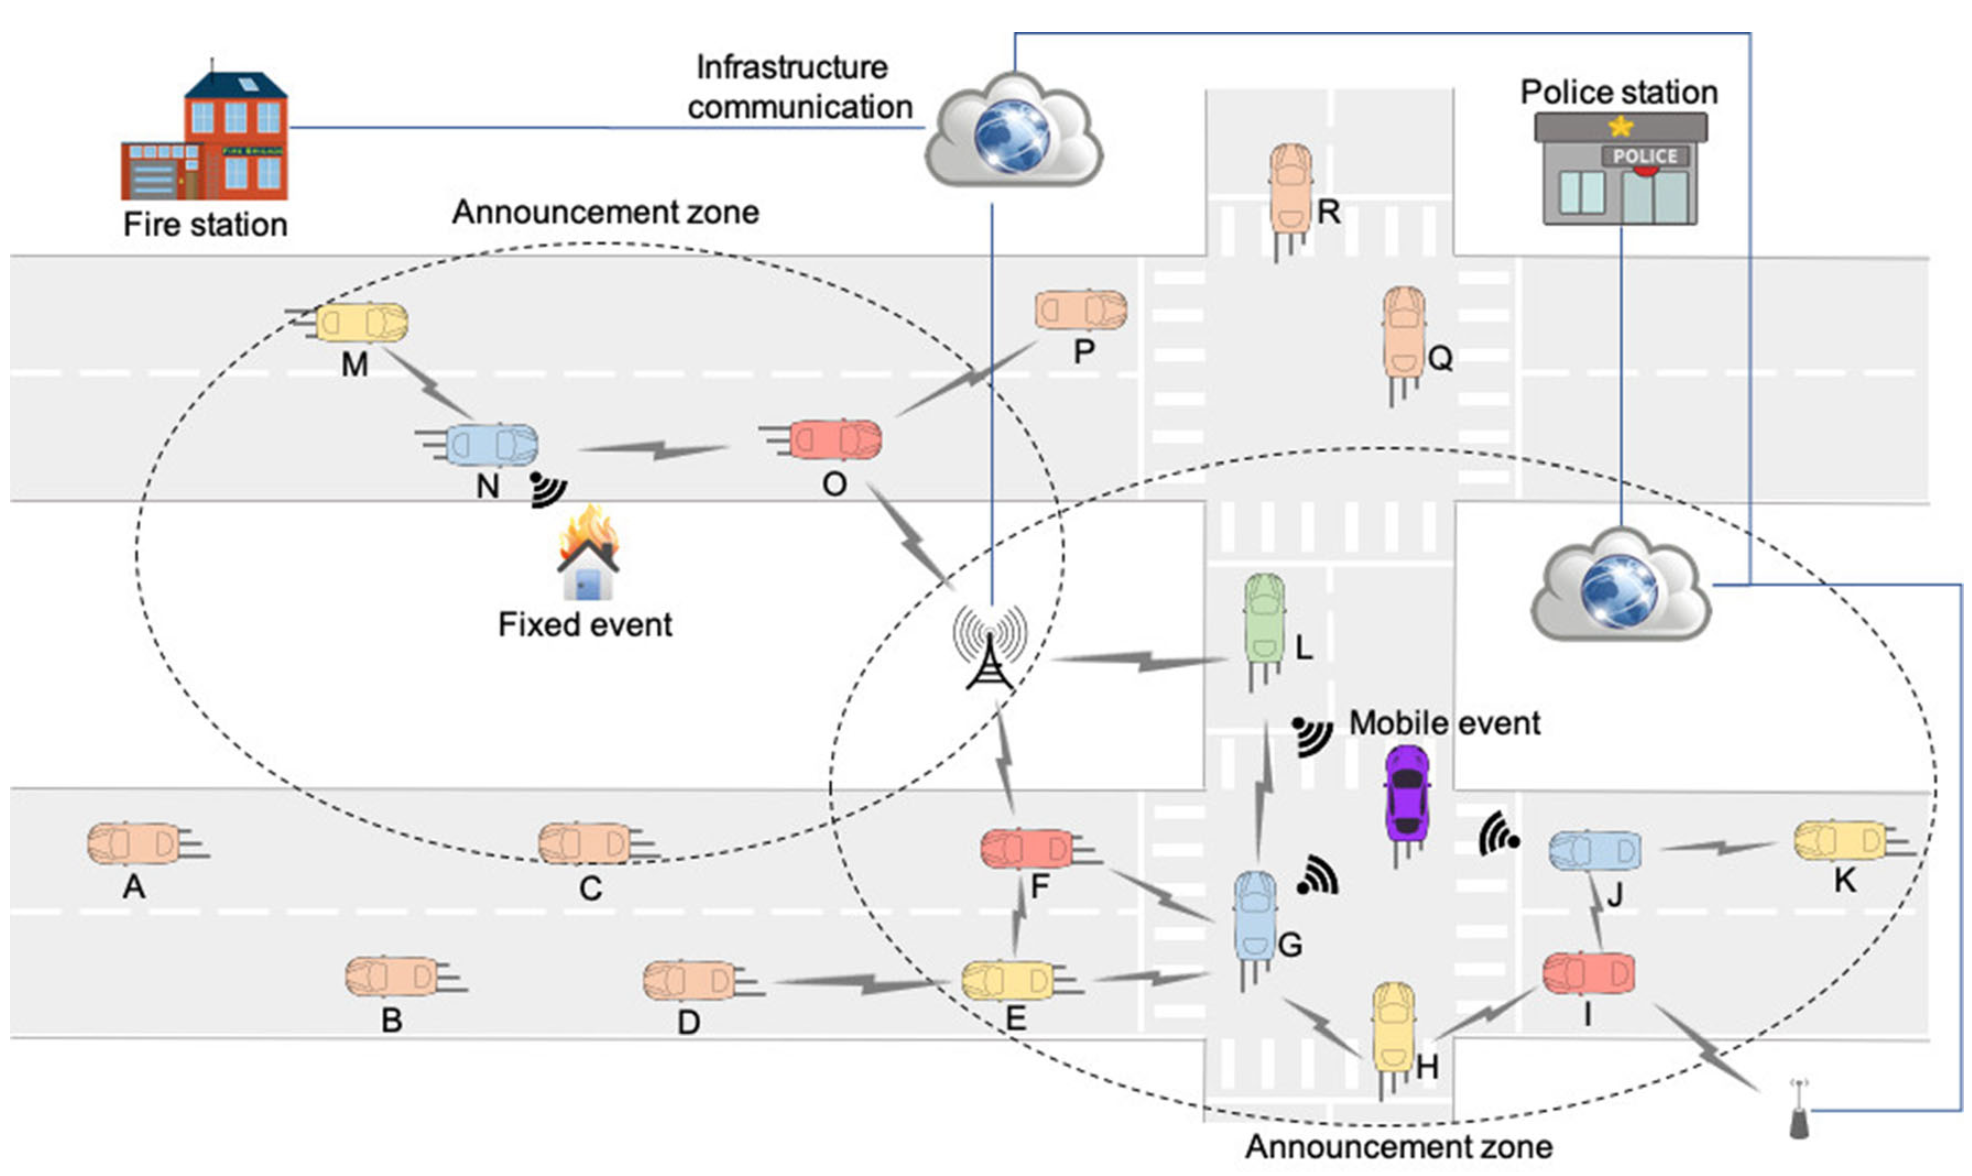
\includegraphics[width=0.85\linewidth]{figs/minuet_cenario.png}}\quad
                \subfloat{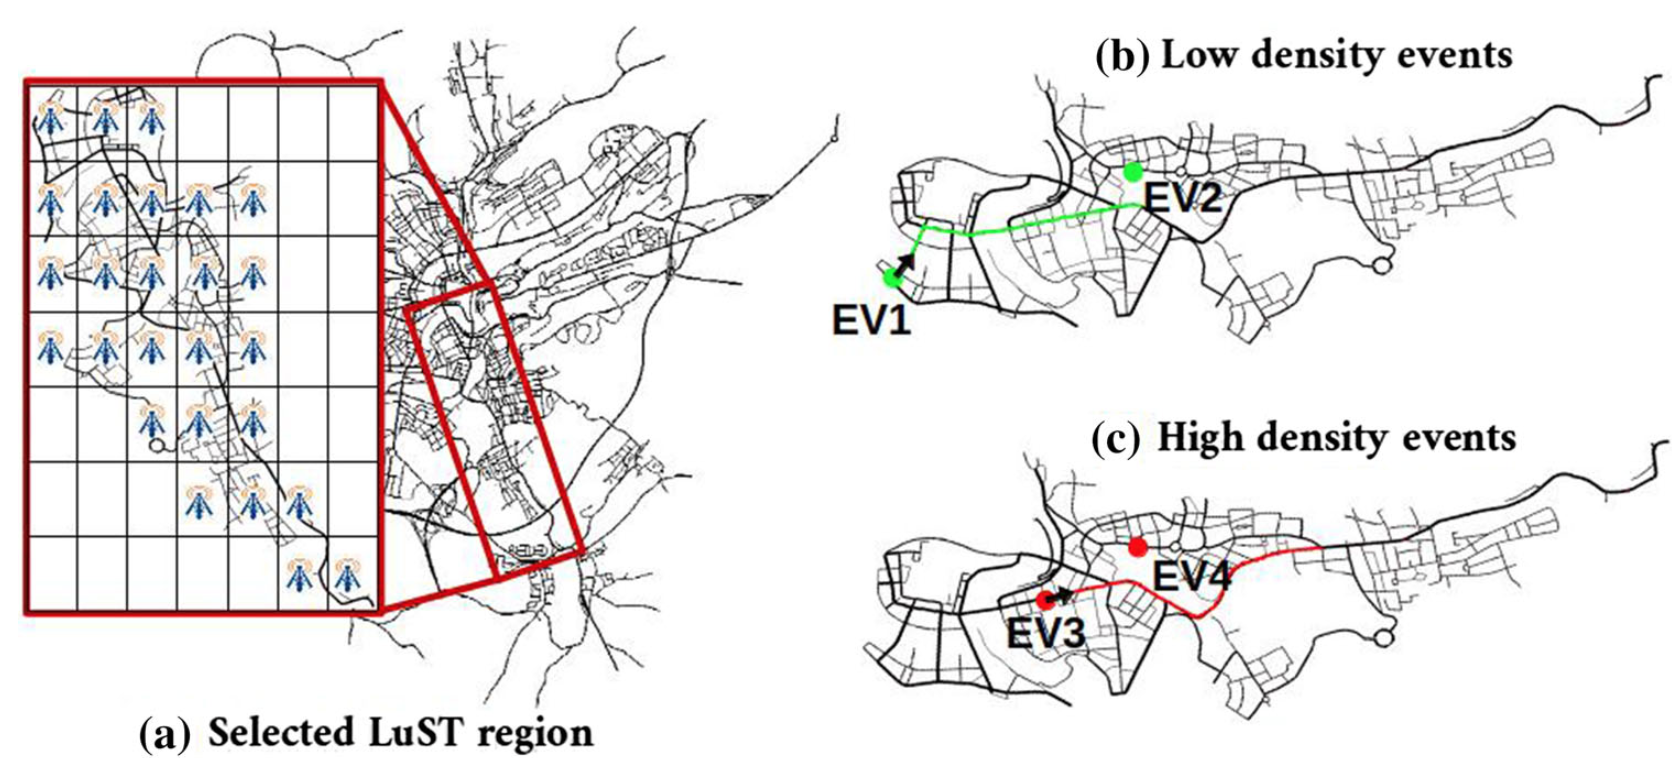
\includegraphics[width=0.75\linewidth]{figs/minuet_lust.png}}
                \caption{Topologia e cenário}
                \label{fig:enter-label}
            \end{figure}    
        \end{column}
        \begin{column}{0.35\textwidth}
            \begin{figure}
                \centering
                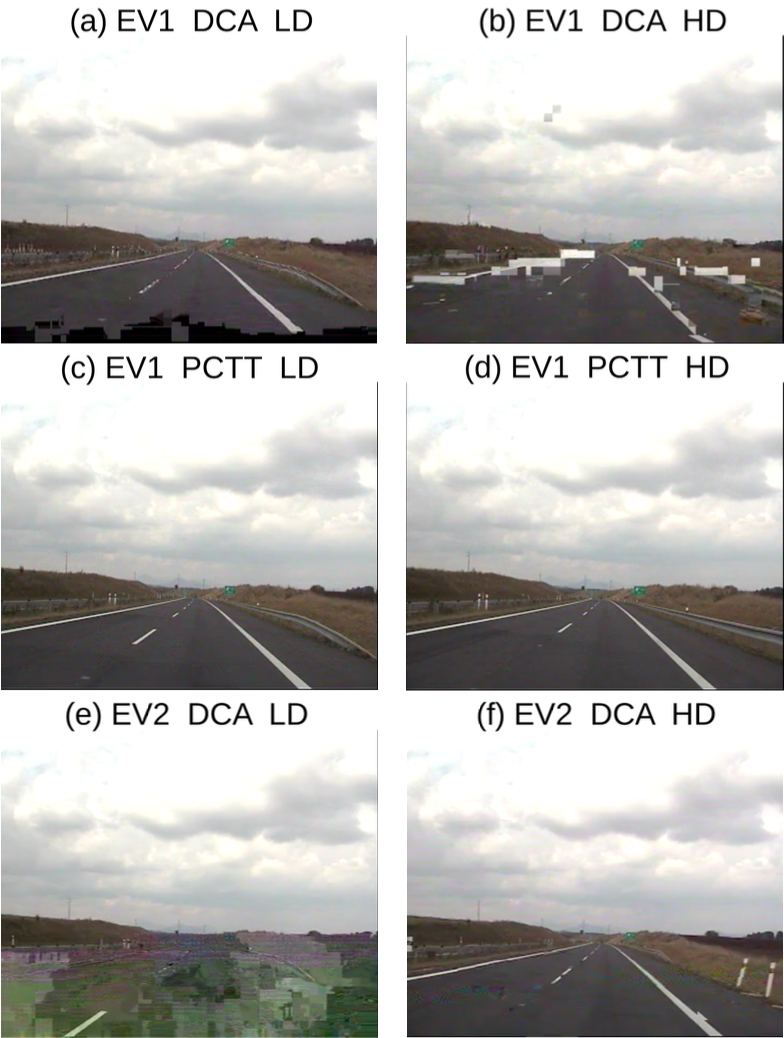
\includegraphics[width=0.9\linewidth]{figs/minuet_video.png}
                \caption{Resultados}
                \label{fig:enter-label}
            \end{figure}
        \end{column}
    \end{columns}
\end{frame}

\begin{frame}{Orquestração e Gerência de \textit{Cloud-Network Slices}\footcite{Rocha2022}}
    \begin{columns}
        \begin{column}{0.5\linewidth}
            \begin{figure}
                \centering
                \subfloat{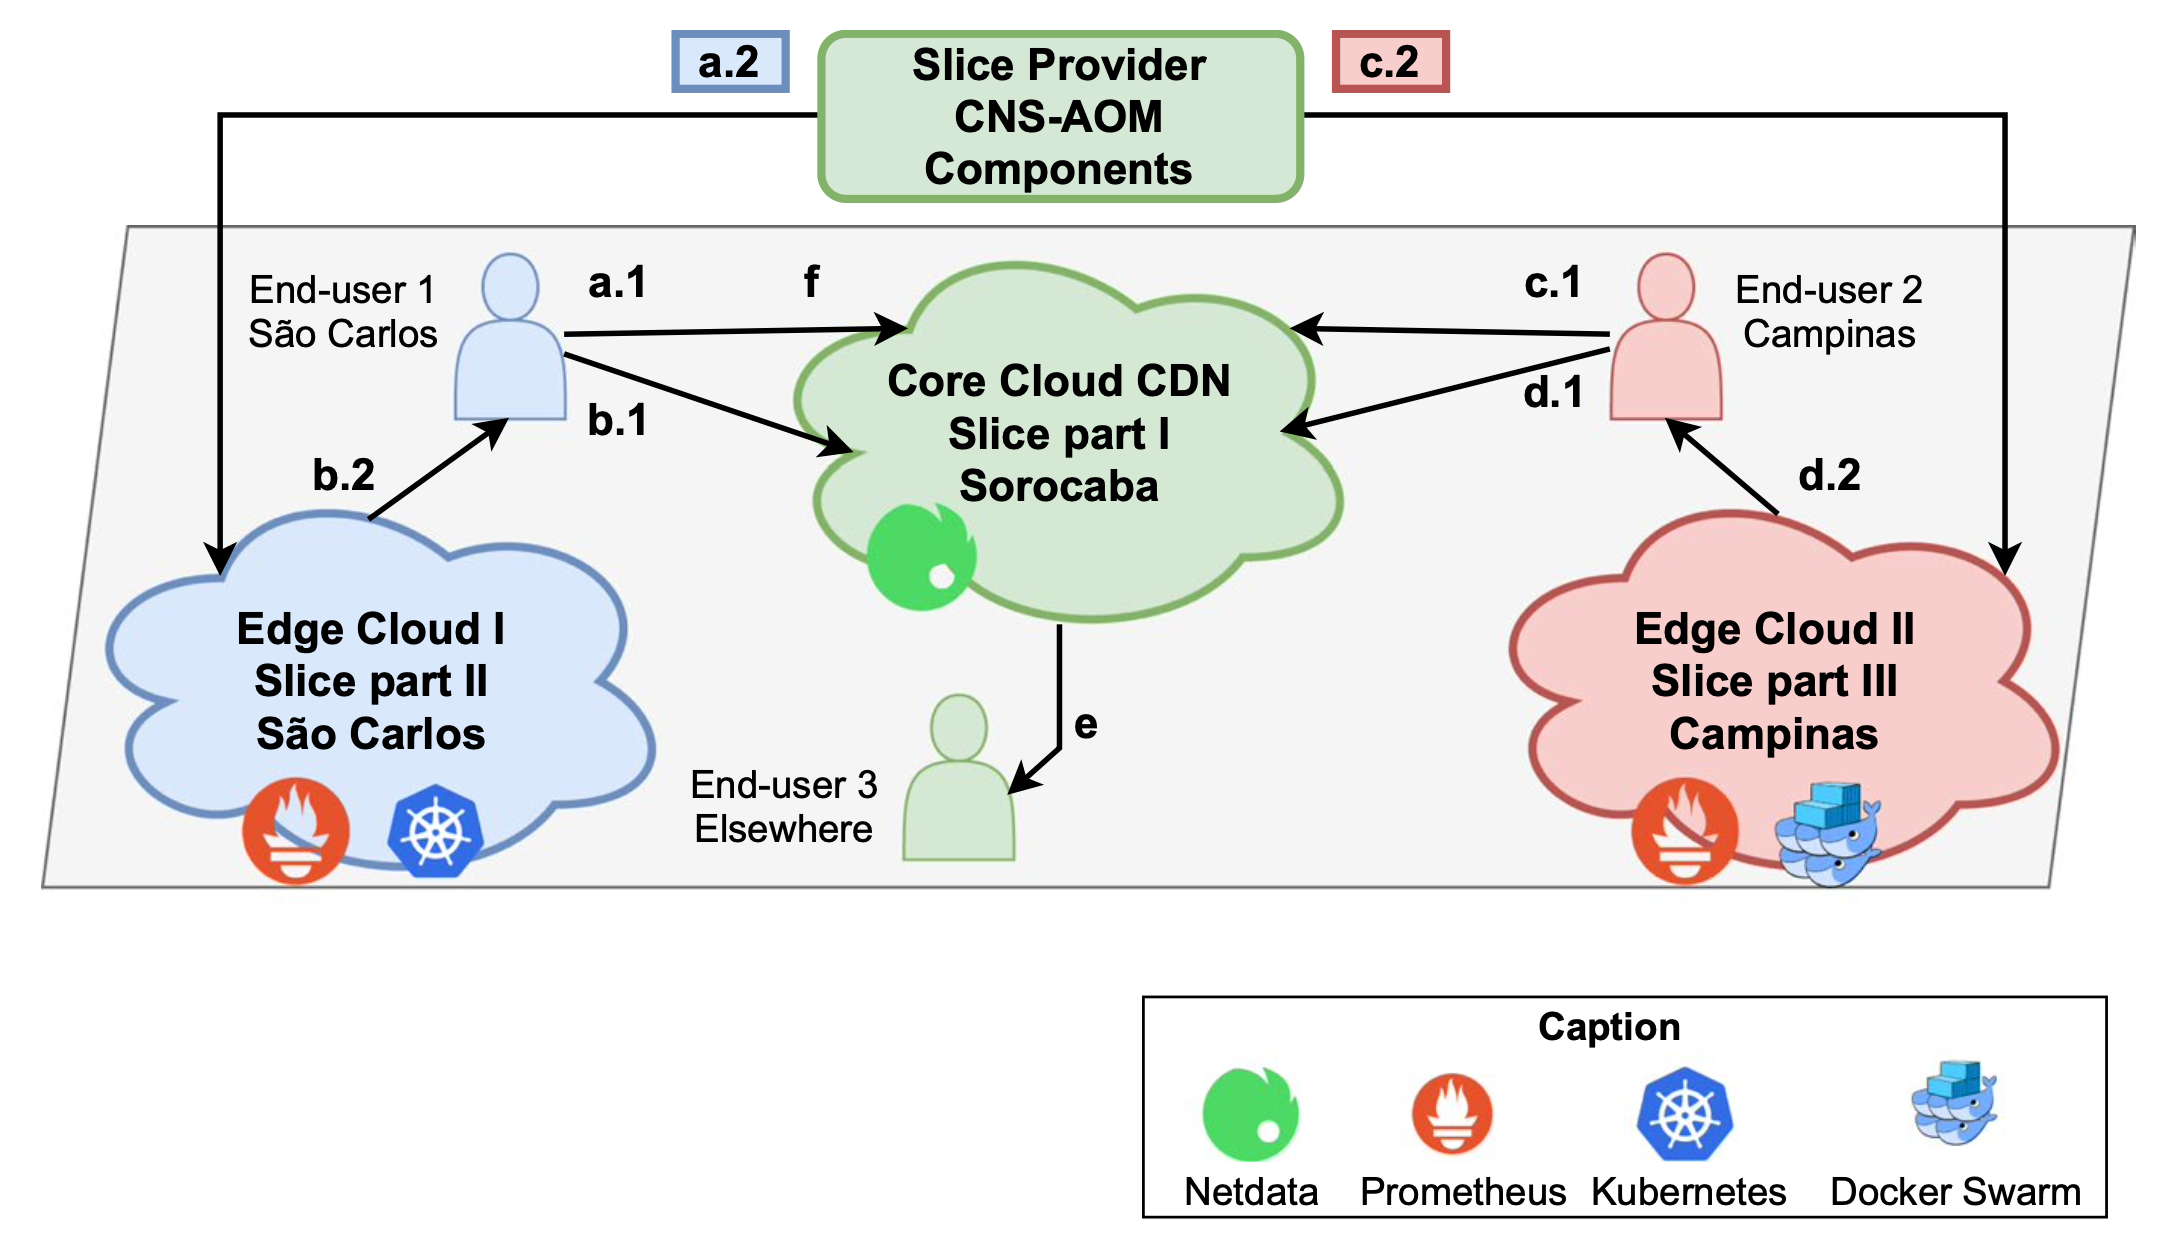
\includegraphics[width=0.9\linewidth]{figs/SEA_POC_VoD.png}}\quad
                \subfloat{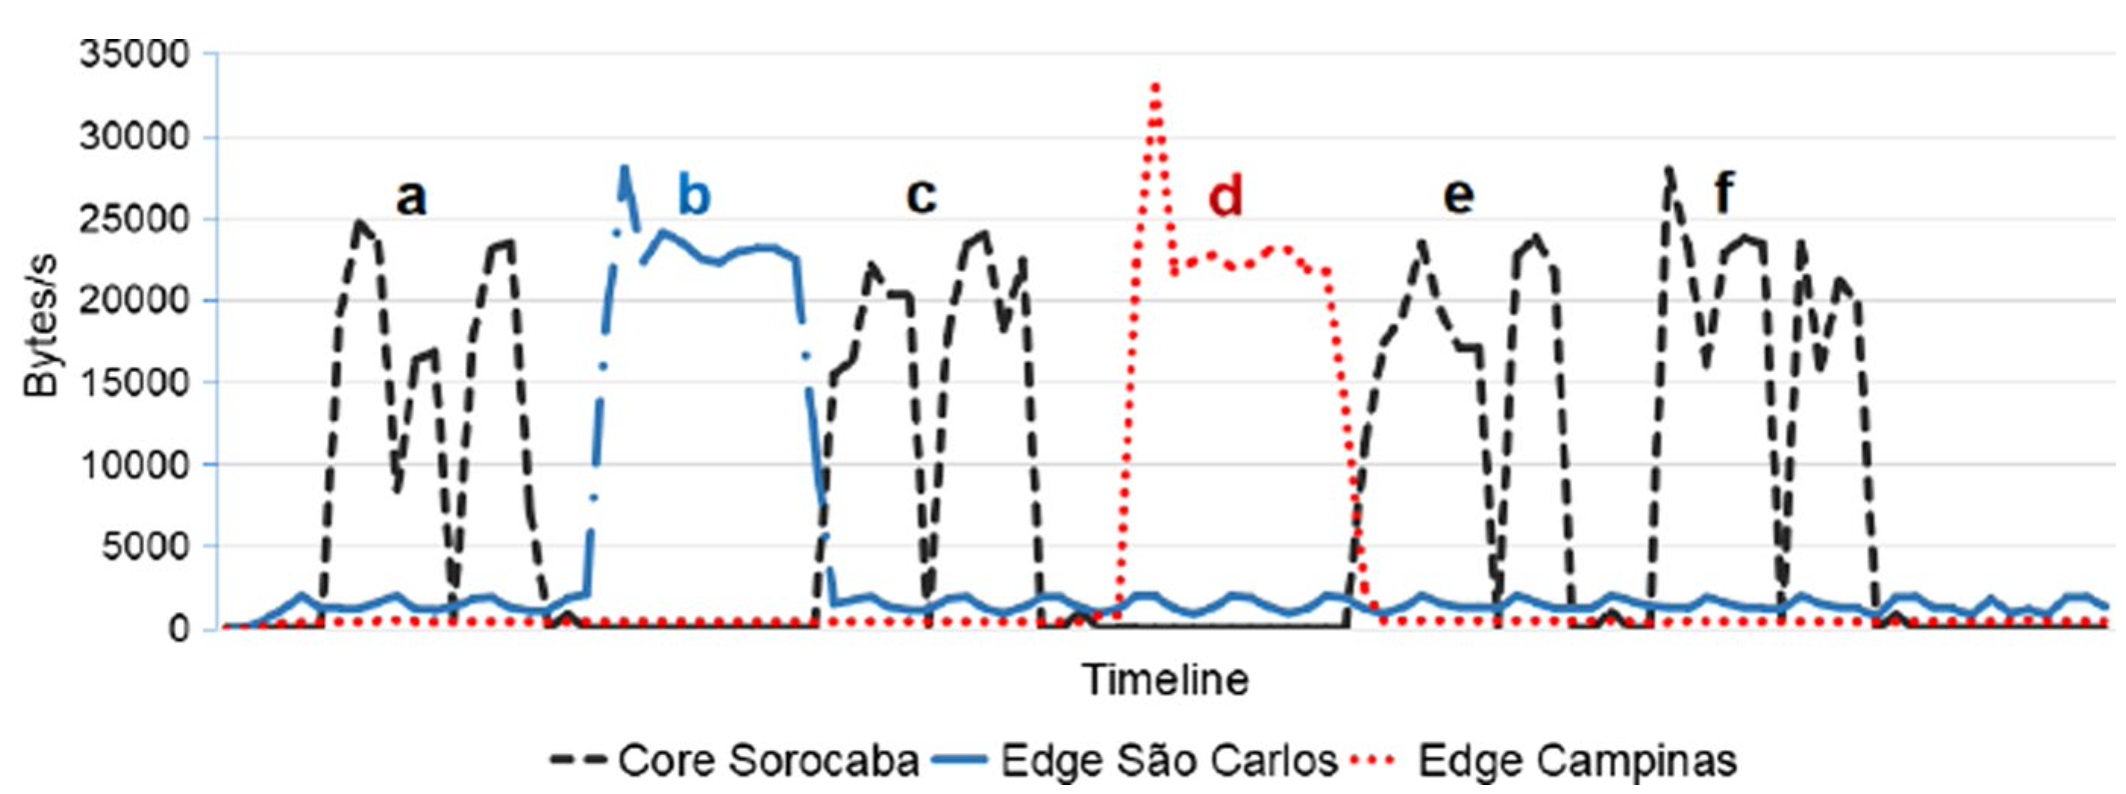
\includegraphics[width=0.9\linewidth]{figs/SEA_Plot_VoD.png}}
                \caption{PoC VoD}
            \end{figure}            
        \end{column}
        \begin{column}{0.5\linewidth}
            \begin{figure}
                \centering
                \subfloat{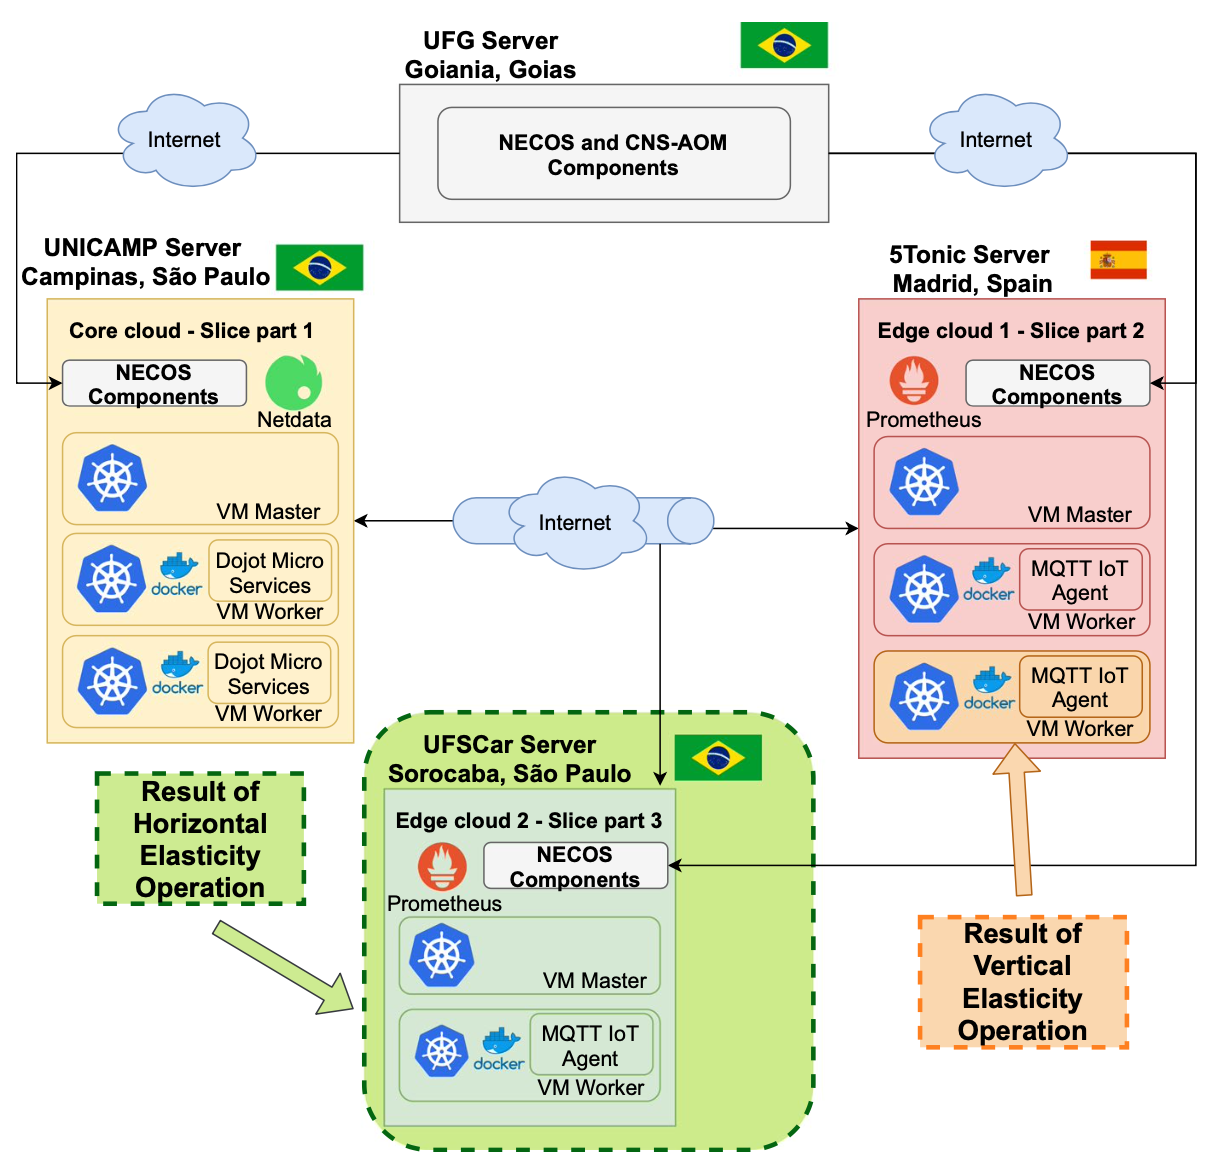
\includegraphics[width=0.8\linewidth]{figs/SEA_POC_IoT.png}}\quad
                \subfloat{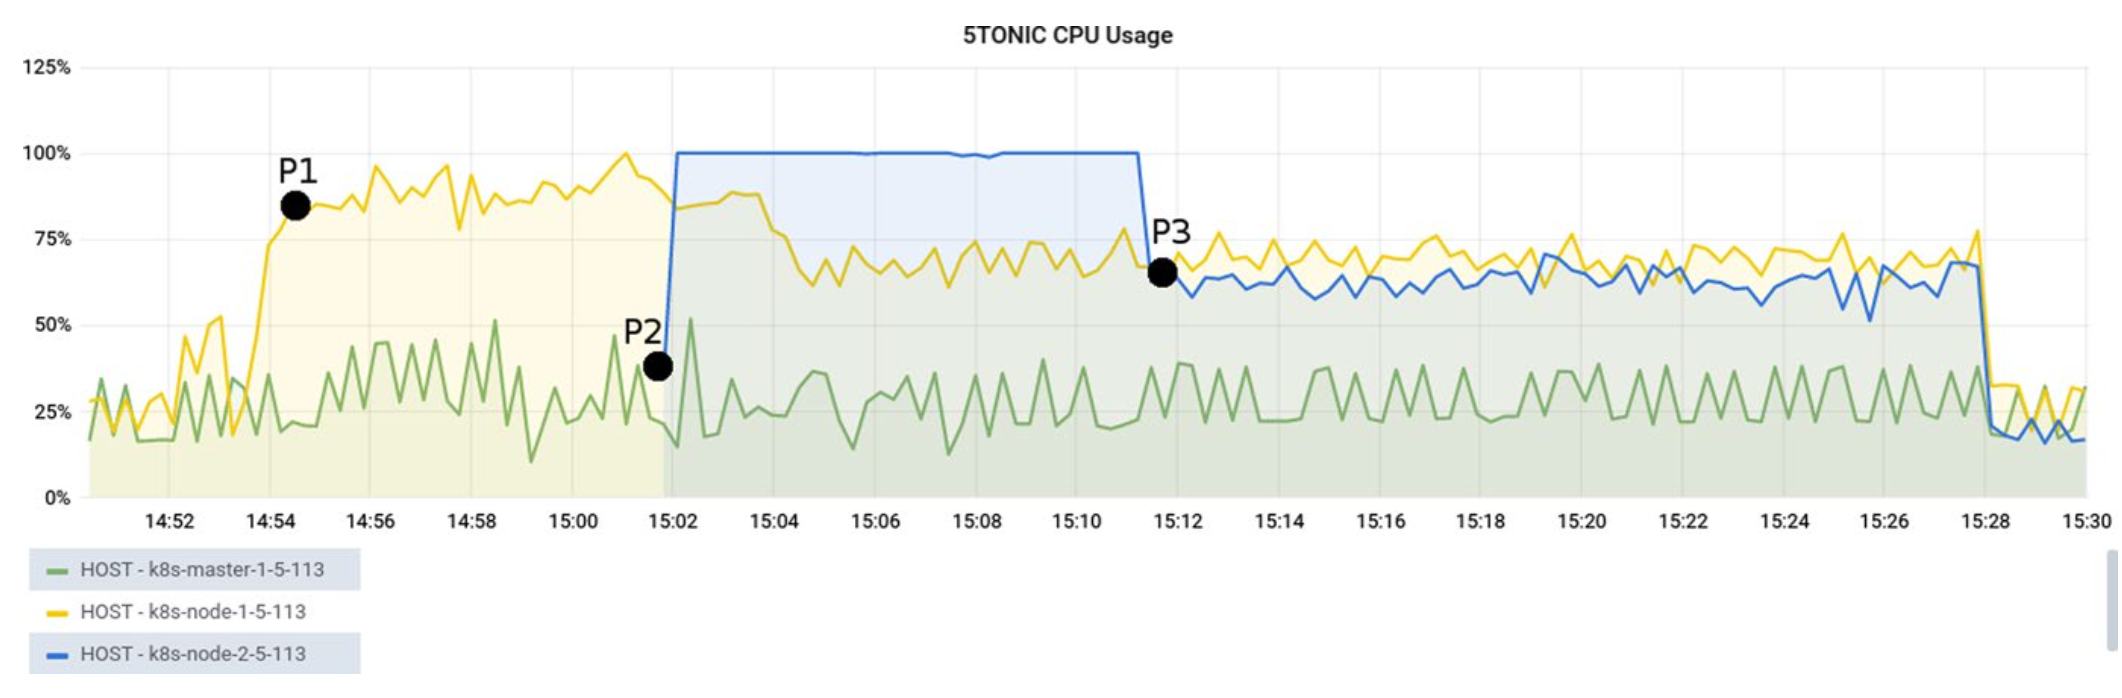
\includegraphics[width=0.8\linewidth]{figs/SEA_Plot_IoT.png}}
                \caption{PoC IoT}
            \end{figure}            
        \end{column}
    \end{columns}
\end{frame}

\begin{frame}{Alocação de Recursos em Redes IoT Multifuncionais\footcite{Silva2024}}
    \begin{figure}
        \centering
        \subfloat{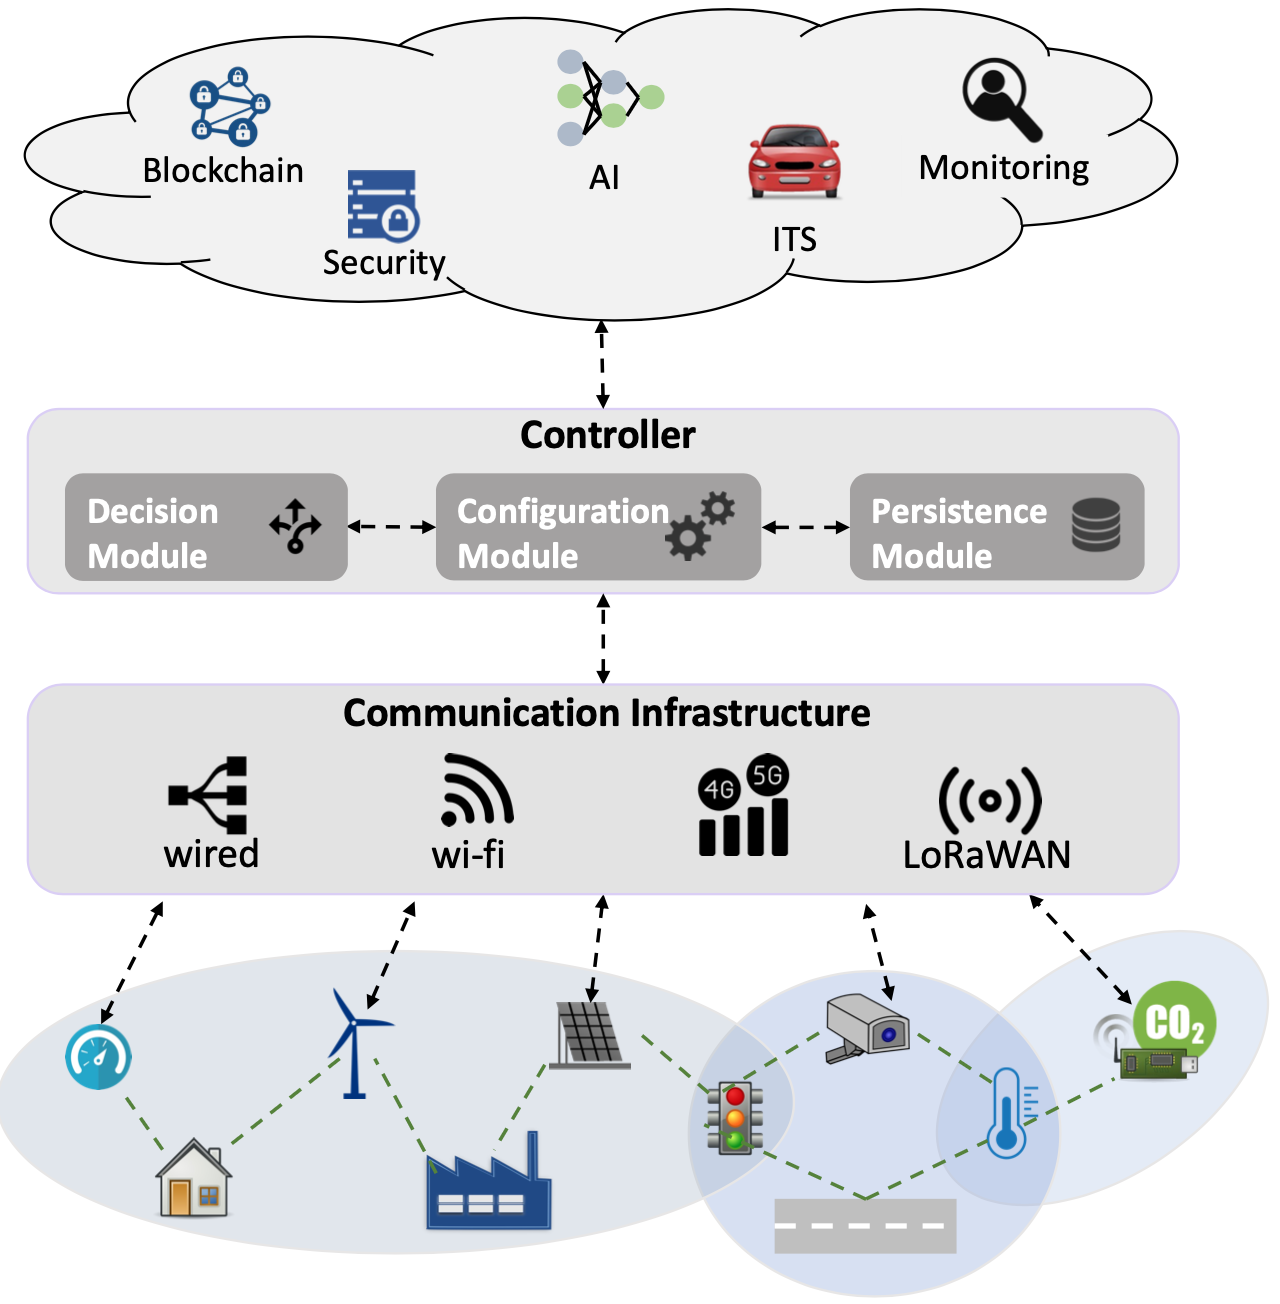
\includegraphics[width=0.5\linewidth]{figs/POSITRON_cenario.png}}
        \hspace{0.5cm}
        \subfloat{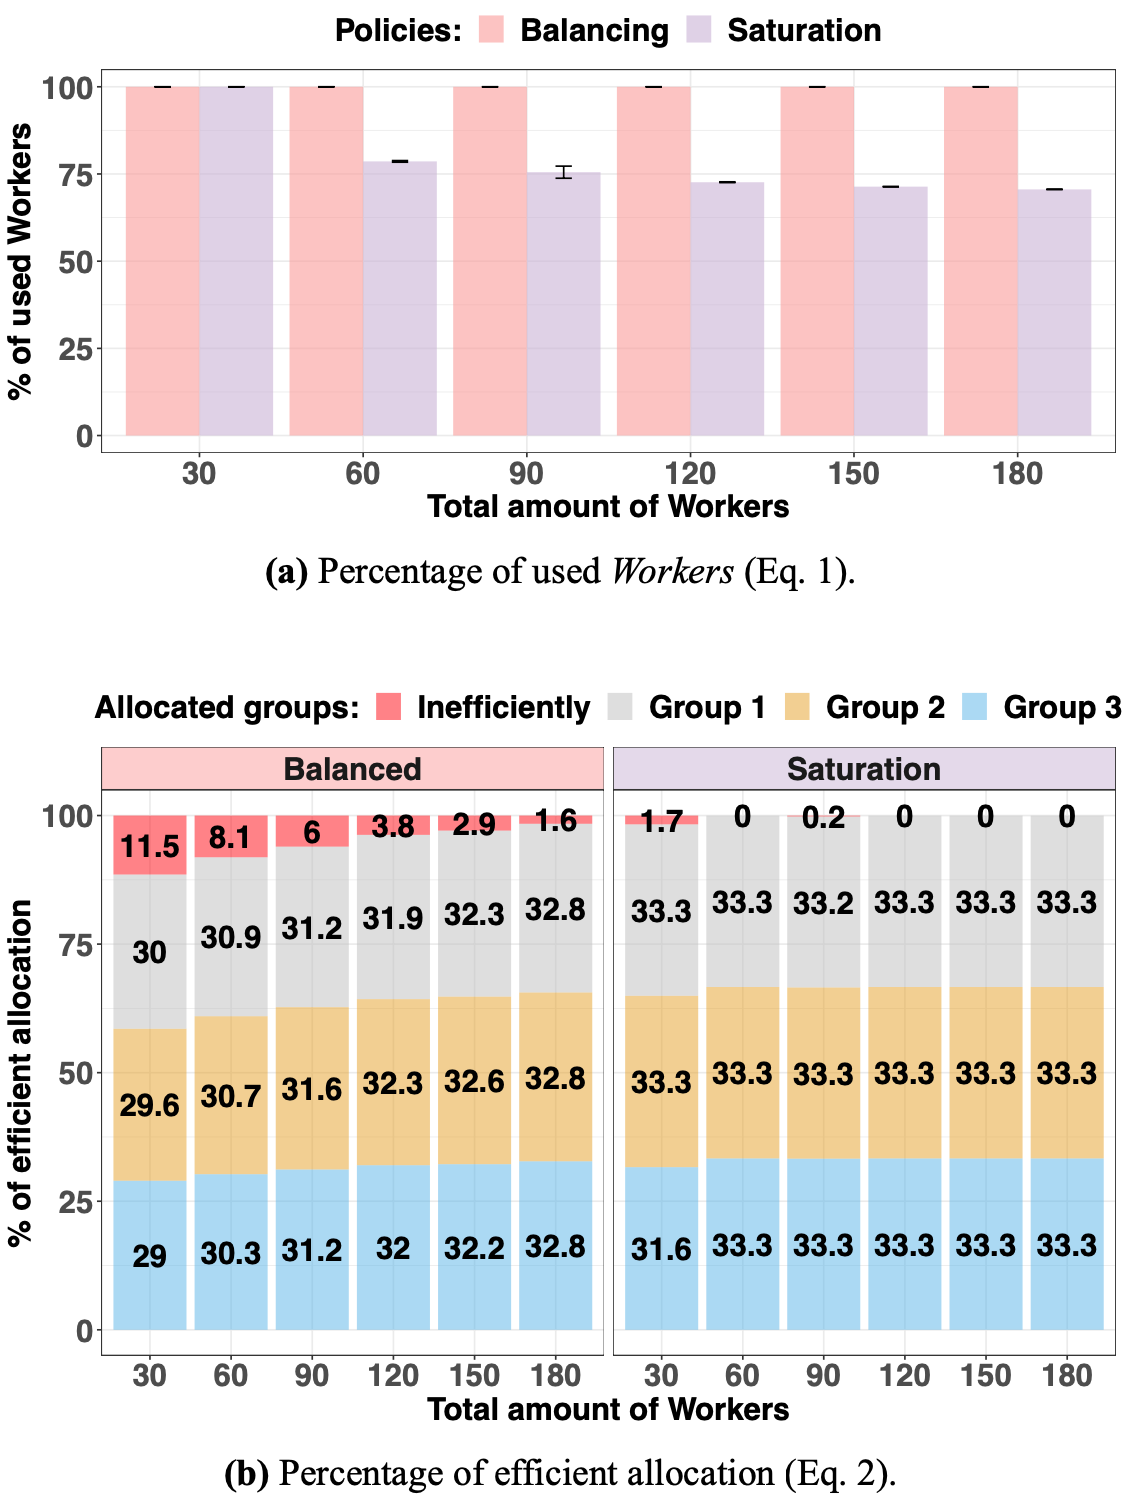
\includegraphics[width=0.4\linewidth]{figs/POSITRON_resultado.png}}
        \caption{Políticas de gerenciamento em redes IoT multifuncionais}
        \label{fig:enter-label}
    \end{figure}
\end{frame}

\begin{frame}{Transmissão de Vídeo em Tempo Real via Rede 5G Privada}
    \begin{columns}
        \begin{column}{0.45\textwidth}
            \begin{itemize}
                \item Implementar ambiente de \textit{testbed} que possibilite experimentação da aplicação de vídeo
                \item Investigar influência da rede de transporte no desempenho das aplicações
                \item Avaliar estratégias para aumento de desempenho na transmissão de vídeo em redes 5G privadas
            \end{itemize}
        \end{column}
        \begin{column}{0.55\textwidth}
            \begin{figure}[htb]
                \centering
                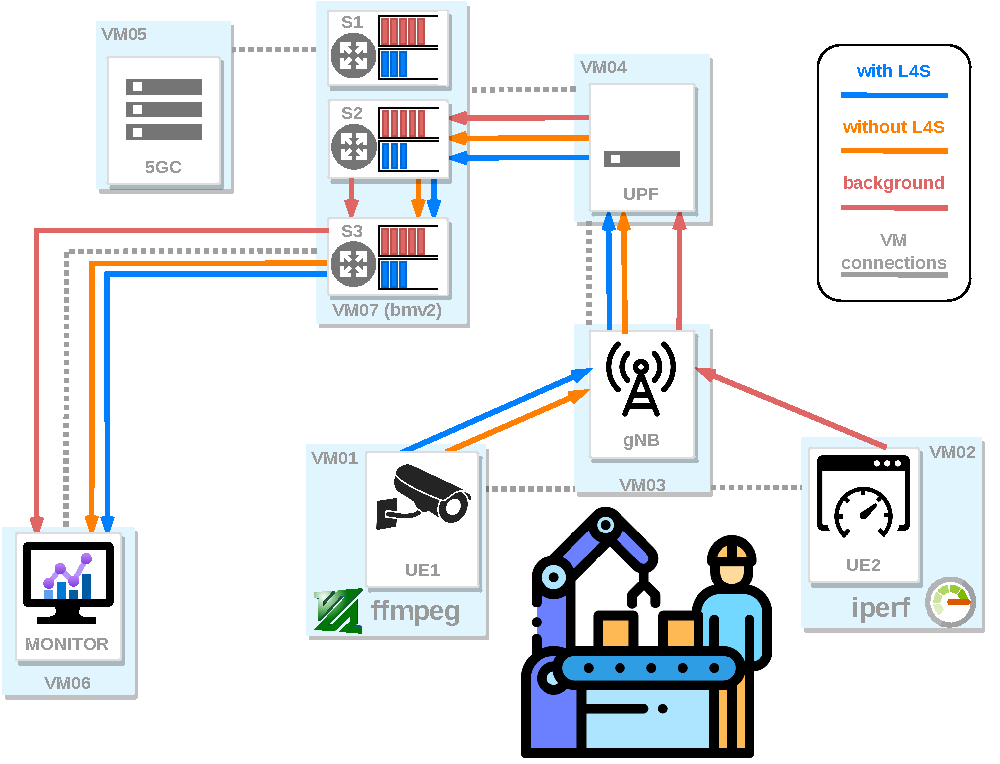
\includegraphics[width=\textwidth]{figs/testbed_5G_privado.pdf}
                \caption{\textit{Testbed} de software com implementação \textit{open source} da rede 5G (autoria própria)}
                \label{fig:setup}
            \end{figure} 
        \end{column}
    \end{columns}
\end{frame}

% Seção 6: Hot Topics
\section{Tópicos Quentes de Pesquisa}
\begin{frame}[allowframebreaks]
    \frametitle{Tópicos Quentes de Pesquisa}
    \begin{itemize}
        \item \textbf{6G e Além}: Exploração de tecnologias para a próxima geração de redes móveis.
        \item \textbf{Inteligência Artificial Integrada}: Aplicação de AI/ML para otimização e automação de redes 5G.
        \item \textbf{Segurança e Privacidade}: Desafios na proteção de dados e na prevenção de ataques cibernéticos em ambientes 5G.
        \item \textbf{Edge Computing Avançado}: Expansão da capacidade de processamento na borda da rede para suportar aplicações em tempo real.
        \item \textbf{Network Slicing Dinâmico}: Desenvolvimento de métodos para alocação e gerenciamento dinâmico de fatias de rede.
        \item \textbf{Integração com IoT Massivo}: Soluções para lidar com a conectividade de bilhões de dispositivos IoT.
        \item \textbf{Ambientes Virtuais e Realidade Aumentada/Virtual}: Potencial do 5G para suportar experiências imersivas de alta qualidade.
    \end{itemize}
\end{frame}

% Seção de Conclusão

\section{Conclusão}
\begin{frame}[allowframebreaks]
    \frametitle{Conclusão}
    \begin{itemize}
        \item A integração SDN/NVF/5G é a base da transformação digital
        \item Flexibilidade e agilidade
        \begin{itemize}
            \item SDN: Controle centralizado e programável da rede.
            \item NFV: Virtualização de funções de rede para rápida implantação e escalabilidade.
        \end{itemize}
        \item Redução de Custos Operacionais
        \begin{itemize}
            \item Menor dependência de hardware proprietário, redução de OPEX e CAPEX.
        \end{itemize}
        \item Automação e Controle em Tempo Real
        \begin{itemize}
            \item SDN: Automação e otimização do tráfego em tempo real.
            \item NFV: Implantação rápida e ajuste de serviços conforme as condições de rede.
        \end{itemize}
    \end{itemize}
\end{frame}

\begin{frame}[allowframebreaks]
\printbibliography
\end{frame}

\begin{comment}
%\AtBeginSection[]
%{
%  \begin{frame}<beamer>
%    \frametitle{Topics}
    %\tableofcontents[currentsection,currentsubsection]
  %\end{frame}
%}

%\section{Histórico - Redes sem Fio}

\begin{frame}
	\frametitle{Agenda}
    \begin{block}{Tópicos da aula}
		\begin{itemize}
			\item O que iremos aprender nesta disciplina
            \vspace{2mm}
            \item O que é um Sistema Operacional (SO) e qual sua utilidade
            \vspace{2mm}
            \item O que devemos saber sobre SOs
		\end{itemize}
	\end{block}
	
\end{frame}

\begin{frame}
	\frametitle{Organização da Disciplina}
    \vspace{-5mm}
    \begin{block}{}
		\begin{itemize}
            \item Principais referências:
            \begin{itemize}
                \item \href{http://pages.cs.wisc.edu/~remzi/OSTEP/}{\textbf{Operating Systems: Three Easy Pieces}} 
                \item An Embedded Software Primer
                \item Sistemas Operacionais de Tempo Real e sua Aplicação em Sistemas Embarcados
                \item Documentação do FreeRTOS para a ESP32
            \end{itemize}
            \vspace{1mm}
            \item Atividades práticas de laboratório
            \begin{itemize}
                \item Programação em C
                \item Programação concorrente (ambiente Linux)
                \item FreeRTOS na ESP32
                \item Curso de Linux (extra)
            \end{itemize}
            \vspace{1mm}
            \item Composição da média final:
            \begin{itemize}
                \item Minitestes com leitura prévia (10\%)
                \item Atividades de laboratório (30\%)
                \item Prova discursiva (30\%)
                \item Projeto Final (30\%)
            \end{itemize}
		\end{itemize}
	\end{block}
	
\end{frame}

\section{O que é um Sistema Operacional?}

\begin{frame}
	\frametitle{O que é um Sistema Operacional?}
    \begin{block}{O que ocorre quando um programa executa?}

	\end{block}
\end{frame}

\begin{frame}
	\frametitle{O que é um Sistema Operacional?}
    \begin{block}{O que ocorre quando um programa executa?}
        \begin{itemize}
        \item Processo simples:
    		\begin{enumerate}
                \item Processador \textbf{busca próxima instrução} na memória
                \vspace{2mm}
                \item \textbf{Decodifica} a instrução
                \vspace{2mm}
                \item \textbf{Executa} a instrução (ex: somar dois números, acessar memória etc)
                \vspace{2mm}
                \item Volta para o passo 1, caso não seja a última instrução
    		\end{enumerate}
        \end{itemize}
	\end{block}
    \begin{alertblock}{Como tornar \textbf{simples de usar?}}
		\begin{itemize}
			\item Camada de software \textbf{intermediária} para:
            \begin{itemize}
                \item Tornar fácil executar \textbf{múltiplos programas em simultâneo}
                \vspace{1mm}
                \item Permitir o \textbf{compartilhamento de recursos} (ex: CPU, memória)
                \vspace{1mm}
                \item Facilitar a \textbf{interação com o hardware}
            \end{itemize}
		\end{itemize}
	\end{alertblock}
\end{frame}

\begin{frame}
	\frametitle{O que é um Sistema Operacional?}

\begin{columns}[T,onlytextwidth]
    \column{0.45\textwidth}
    \begin{tikzpicture} \node (A) at (0,6) [draw,orange,ultra thick,minimum width=4cm,minimum height=1.5cm] {Usuário}; \node (B) at (0,4) [draw,green,ultra thick,minimum width=4cm,minimum height=1.5cm] {Aplicações}; \node (C) at (0,2) [draw,blue,ultra thick,minimum width=4cm,minimum height=1.5cm] {Sistema Operacional}; \node (D) at (0,0) [draw,brown,ultra thick,minimum width=4cm,minimum height=1.5cm] {Hardware};
    
    \path (A.south) -- (A.south west) coordinate[pos=0.5] (a00); \path (B.north) -- (B.north west) coordinate[pos=0.5] (b01); \draw[latex-] (a00) -- (b01);
    
    \path (B.south) -- (B.south west) coordinate[pos=0.5] (b00); \path (C.north) -- (C.north west) coordinate[pos=0.5] (c01); \draw[latex-] (b00) -- (c01);
    
    \path (C.south) -- (C.south west) coordinate[pos=0.5] (c00); \path (D.north) -- (D.north west) coordinate[pos=0.5] (d01); \draw[latex-] (c00) -- (d01);
    
    \path (A.south) -- (A.south east) coordinate[pos=0.5] (a10); \path (B.north) -- (B.north east) coordinate[pos=0.5] (b11); \draw[latex-] (b11) -- (a10);
    
    \path (B.south) -- (B.south east) coordinate[pos=0.5] (b10); \path (C.north) -- (C.north east) coordinate[pos=0.5] (c11); \draw[latex-] (c11) -- (b10);
    
    \path (C.south) -- (C.south east) coordinate[pos=0.5] (c10); \path (D.north) -- (D.north east) coordinate[pos=0.5] (d11); \draw[latex-] (d11) -- (c10);
    
    \end{tikzpicture}
   
    \column{0.6\textwidth}
    \begin{alertblock}{SO é um \textit{middleware} entre aplicações e o hardware}
        \begin{itemize}
            \item Provê \textbf{interfaces padronizadas} para os recursos
            \vspace{1mm}
            \item \textbf{Gerencia} o hardware
            \vspace{1mm}
            \item Realiza \textbf{orquestração} de processos em execução
            \vspace{1mm}
            \item Responde a \textbf{requisições de acesso a recursos}
            \vspace{1mm}
            \item Trata o \textbf{controle de acesso}
        \end{itemize}
    \end{alertblock}
\end{columns}
\end{frame}



\begin{frame}
	\frametitle{Primeiro Papel do SO $\rightarrow$ Interface padrão}
        \begin{block}{Prover \textbf{interfaces comuns} para as aplicações}
                \begin{itemize}
                    \item Abstrai diferenças entre hardwares distintos
                    \vspace{1mm}
                    \item Disponíveis por meio de bibliotecas
                \end{itemize}
                %\vspace{1mm}
                %\item Gerencia os recursos (CPU, memória, disco etc)
    	\end{block}
     \begin{alertblock} {Exemplo}
         \begin{itemize}
            \item Pode-se utilizar diferentes placas de rede ou diferentes tipos de dispositivos de armazenamento, mas os programas utilizam a mesma API para interagir com o hardware
            \begin{itemize}
                \item Ex: enviar ou receber pacotes na rede
                \vspace{1mm}
                \item Ex2: ler ou escrever em arquivos
            \end{itemize}
         \end{itemize}
     \end{alertblock}
\end{frame}

\begin{frame}
	\frametitle{Segundo Papel do SO $\rightarrow$ Gerenciamento de recursos}
        \begin{block}{O SO \textbf{compartilha} os recursos entre as aplicações}
                \begin{itemize}
                    \item Isolamento $\rightarrow$ \textbf{protege} as aplicações umas das outras
                    \vspace{1mm}
                    \item Escalonamento $\rightarrow$ \textbf{provê acesso} justo e eficiente aos recursos
                    \vspace{1mm}
                    \item Limita $\rightarrow$ \textbf{divide o acesso} aos recursos
                \end{itemize}
                %\vspace{1mm}
                %\item Gerencia os recursos (CPU, memória, disco etc)
    	\end{block}

\end{frame}

\begin{frame}\frametitle{SO $\rightarrow$ três ``pedaços''}

O projeto de um SO pode ser dividido em três pilares\\
\vspace{4mm}
\begin{tikzpicture} \draw [orange, ultra thick] (0,0) rectangle (2,4); \node[text width=3cm, rotate=90] at (1, 2.5) {Virtualização}; \draw [blue, ultra thick] (3,0) rectangle (5,4); \node[text width=3cm, rotate=90] at (4, 2.5) {Concorrência}; \draw [green, ultra thick] (6,0) rectangle (8,4); \node[text width=3cm, rotate=90] at (7, 2.5) {Persistência};

%\draw [red, ultra thick] (0,4.5) -- (8,4.5); \draw [red, ultra thick] (0,4.5) -- (4,6); \draw [red, ultra thick] (4,6) -- (8,4.5); \node[text width=3cm] at (5, 5) {Segurança};

\end{tikzpicture}
\end{frame}

\begin{frame}\frametitle{Primeiro pilar $\rightarrow$ Virtualização}

     \begin{alertblock} {O SO ``virtualiza'' o hardware}
         \begin{itemize}
            \item As aplicações executam com a ``ilusão'' de possuírem \textbf{acesso exclusivo} ao hardware
         \end{itemize}
     \end{alertblock}

     \begin{block}{Alguns desafios surgem}
         \begin{itemize}
             \item \textbf{O que executar} em um dado momento?
             \vspace{1mm}
             \item \textbf{Como dividir os recursos} sem causar interferência entre programas em execução diferentes?
             \vspace{1mm}
             \item O SO precisa de \textbf{mecanismos} e \textbf{políticas}
         \end{itemize}
     \end{block}

\end{frame}

\begin{frame}\frametitle{Primeiro pilar $\rightarrow$ Virtualizando a CPU}

    \begin{figure}
        \centering
        \includegraphics[width=0.9\textwidth]{figs/codecap1_1.png}
        \tiny \\Fonte: Operating Systems: Three Easy Pieces. Remzi H. Arpaci-Dusseau and Andrea C. Arpaci-Dusseau. Arpaci-Dusseau Books. November, 2023 (Version 1.10)
        \end{figure}

\end{frame}

\begin{frame}\frametitle{Primeiro pilar $\rightarrow$ Virtualizando a CPU}
    Criando um processo (programa em execução)\\
    \vspace{1mm}
    \begin{figure}
        \centering
        \includegraphics[width=0.7\textwidth]{figs/runningcodecap1_1.png}
         \tiny \\Fonte: Operating Systems: Three Easy Pieces. Remzi H. Arpaci-Dusseau and Andrea C. Arpaci-Dusseau. Arpaci-Dusseau Books. November, 2023 (Version 1.10)
    \end{figure}

\end{frame}

\begin{frame}\frametitle{Primeiro pilar $\rightarrow$ Virtualizando a CPU}
    Criando vários processos (programas em execução)\\
    \vspace{1mm}
    \begin{figure}
        \centering
        \includegraphics[width=0.85\textwidth]{figs/runningcodecap1_2.png}
         \tiny \\Fonte: Operating Systems: Three Easy Pieces. Remzi H. Arpaci-Dusseau and Andrea C. Arpaci-Dusseau. Arpaci-Dusseau Books. November, 2023 (Version 1.10)
    \end{figure}

\end{frame}

\begin{frame}\frametitle{Primeiro pilar $\rightarrow$ Virtualizando a Memória}
    \begin{block}{A memória física é um \textbf{array de bytes}}
        \begin{itemize}
            \item Os programas mantém \textbf{todos os seus dados} em memória durante a execução
            \begin{itemize}
                \item \textit{load} $\rightarrow$ Especifica um endereço para obter o dado
                \vspace{1mm}
                \item \textit{store} $\rightarrow$ Especifica um endereço e um dado para ser escrito
            \end{itemize}
            \vspace{2mm}
            \item O SO provê um \textbf{espaço de endereçamento virtual} para um programa em execução
        \end{itemize}
        
    \end{block}

\end{frame}

\begin{frame}\frametitle{Primeiro pilar $\rightarrow$ Virtualizando a Memória}
    \begin{figure}
        \centering
        \includegraphics[width=0.85\textwidth]{figs/codecap1_2.png}
         \tiny \\Fonte: Operating Systems: Three Easy Pieces. Remzi H. Arpaci-Dusseau and Andrea C. Arpaci-Dusseau. Arpaci-Dusseau Books. November, 2023 (Version 1.10)
    \end{figure}
\end{frame}

\begin{frame}\frametitle{Primeiro pilar $\rightarrow$ Virtualizando a Memória}
    Verificando o endereço da memória alocada\footnote{\tiny Para este exemplo funcionar dessa forma, é necessário desabilitar a aleatorização do espaço de endereçamento.}\\
    \vspace{1mm}
    \begin{figure}
        \centering
        \includegraphics[width=0.85\textwidth]{figs/runningcodecap1_2_1.png}
         \tiny \\Fonte: Operating Systems: Three Easy Pieces. Remzi H. Arpaci-Dusseau and Andrea C. Arpaci-Dusseau. Arpaci-Dusseau Books. November, 2023 (Version 1.10)
    \end{figure}
\end{frame}

\begin{frame}\frametitle{Segundo pilar $\rightarrow$ Concorrência}
    \begin{block}{O SO gerencia \textbf{várias coisas ao mesmo tempo}}
        \begin{itemize}
            \item Vários processos executam em simultâneo
            \vspace{1mm}
            \item Pode ser necessário realizar comunicação entre processos
        \end{itemize}
        
    \end{block}
    \begin{alertblock}{Pode haver concorrência dentro do mesmo processo (\textit{multi-thread})}

    \end{alertblock}
    \vspace{2mm}
    \begin{figure}
        \centering
        \includegraphics[width=0.65\textwidth]{figs/programmerhumor-io-programming-memes-linux-memes-9a74c163a7cd584.png}
        \tiny \\ Fonte: \url{https://programmerhumor.io/programming-memes/multithreading-in-a-nutshell/}
    \end{figure}
\end{frame}


\begin{frame}\frametitle{Segundo pilar $\rightarrow$ Concorrência}
    \begin{figure}
        \centering
        \includegraphics[width=0.6\textwidth]{figs/codecap1_3.png}
         \tiny \\Fonte: Operating Systems: Three Easy Pieces. Remzi H. Arpaci-Dusseau and Andrea C. Arpaci-Dusseau. Arpaci-Dusseau Books. November, 2023 (Version 1.10)
    \end{figure}
\end{frame}

\begin{frame}\frametitle{Terceiro pilar $\rightarrow$ Persistência}
    \begin{block}{Memória principal é \textbf{volátil}}
        \end{block}

        
    \begin{alertblock}{É necessário hardware e software para prover armazenamento persistente}
        \begin{itemize}
            \item Hardware $\rightarrow$ Dispositivo de I/O como disco rígido ou SSD (\textit{solid-state driver}) 
            \vspace{1mm}
            \item Software
            \begin{itemize}
                \item Driver de disco
                \vspace{1mm}
                \item Sistema de arquivo para gerenciar o disco (abstrai como o arquivo é armazenado)
            \end{itemize}
        \end{itemize}
    \end{alertblock}
\end{frame}

\begin{frame}\frametitle{Terceiro pilar $\rightarrow$ Persistência}
    Cria um arquivo (\textit{/tmp/file}) que contém a string ``hello world''\\
    \vspace{1mm}
    \begin{figure}
        \centering
        \includegraphics[width=0.7\textwidth]{figs/codecap1_4.png}
         \tiny \\Fonte: Operating Systems: Three Easy Pieces. Remzi H. Arpaci-Dusseau and Andrea C. Arpaci-Dusseau. Arpaci-Dusseau Books. November, 2023 (Version 1.10)
    \end{figure}
\end{frame}

\begin{frame}\frametitle{Breve Histórico}
    \begin{block}{Evolução do sistemas operacionais}
        \begin{enumerate}
            \item \textbf{Biblioteca} para funções de uso comum
            \vspace{1mm}
            \item Evolução de chamadas de procedimento para \textbf{chamadas de sistema}
            \begin{itemize}
                \item Delimitação do \textbf{nível de privilégio} para execução
                \vspace{1mm}
                \item OS executa com privilégio mais elevado que as aplicações
            \end{itemize}
            \vspace{1mm}
            \item Execução \textbf{concorrente} de processos (multiprogramação)
            \begin{itemize}
                \item \textbf{Chaveamento} entre diferentes processos
                \vspace{1mm}
                \item Aumento da \textbf{eficiência} no uso do processador
                \vspace{1mm}
                \item Necessidade de \textbf{isolamento} entre os processos
                \vspace{1mm}
                \item Novos \textbf{desafios de concorrência} surgem
            \end{itemize}
        \end{enumerate}
    \end{block}
\end{frame}
\end{comment}

\end{document}
